\chapter{Literature review}\label{ch:literature-review}

It is a widely accepted practice to conduct a systematic literature review to \enquote{identify research relevant to a specific research question}~\cite{kitchenham_guidelines_2007}.
The methodology of this review has been based on guidelines published by Kitchenham and Charters~\cite{kitchenham_guidelines_2007} and Neiva and L.~S.~Silva~\cite{neiva_systematic_2016}.
It will cover three phases, described in subsequent sections: preparation and planning (described in section~\ref{sec:planning-and-preparation-for-review}), execution and reporting (described in section~\ref{sec:conducting-and-reporting-the-search}), and discussion of results (section~\ref{sec:review-discussion-of-results}).

\section[Planning and preparation]{Planning and preparation for review}\label{sec:planning-and-preparation-for-review}

\subsection{Defining research questions and justifying the review}\label{subsec:defining-research-questions-and-justifying-the-review}

There have been several surveys of UIDLs conducted in the past~\cite{Souchon2003, guerrero_garcia_theoretical_2009, guerrero_garcia_theoretical_2011, Jovanovic2013}.
They mention the expressiveness requirement directly or indirectly (\enquote{amount of tags, coverage of concepts}) in their comparisons;
however, they are not systematic and well-documented.
The latest review has been published in 2013 and there does not seem to exist a more recent overview.
Additionally, the documents have been focused on XML-based languages and did not research any other forms of representing user interfaces.

A systematic review by Ruiz et al~\cite{Ruiz2018} defines 10 criteria for evaluation of MBUID environments.
Two of them (code generation and design flexibility) are relevant to the purposes of this thesis.
However, the paper only provides a general, nonspecific methodology for evaluation.
Additionally, it does not focus on representations themselves and does not include approaches from later than 2015.

\subsection{Defining search criteria}\label{subsec:defining-search-criteria}
First, keywords and synonyms relevant to identifying existing UI representations were first identified:
\begin{itemize}
    \item \textbf{abstract}/universal/generic/declarative/intermediate/polymorphic/(platform-)independent/(device-)independent/multi-platform/multi-device -- \textit{(terms related to non-direct descriptions)}
    \item \textbf{user interface}/UI -- \textit{(terms related to user interfaces)}
    \item \textbf{representation}/(meta-)model/language/specification/description -- \textit{(synonyms of \enquote{representation})}
\end{itemize}
Based on these keywords, it was possible to formulate a search string: synonyms and their different spellings are connected using a Boolean \texttt{OR} operator and groups of synonyms are connected using an \texttt{AND} operator.
The initial search string was used to perform a tentative search;
it helped validate that the returned results contain relevant papers and helped refine the search string by adding more synonyms of selected keywords.
Additionally, the term \emph{user interface description language} and its initialism \emph{UIDL} are appended to the search string using \texttt{OR}s as a recognizable term that would not be matched by the previously described conjunction of keywords.
The final search string is shown in Listing~\ref{lst:general-search-string-rq-1}.
\begin{lstlisting}[label=lst:general-search-string-rq-1,caption=The search string, basicstyle=\ttfamily]
(
  (UI OR "user interface")
  AND
  (
    abstract OR declarative OR intermediate OR universal OR polymorphic OR
    generic OR independent OR device-independent OR multi-platform OR multi-device
  )
  AND
  (
    description OR describing OR model OR modelling OR
    metamodel OR meta-model OR "meta model" OR
    language OR representation OR specification OR specifying
  )
)
OR ("user interface description language" OR UIDL)
    \label
\end{lstlisting}

To improve and narrow down the results of the searches, additional criteria are to be used:
\begin{samepage}
\begin{itemize}
    \item papers should concern only the field of computer science
    \item papers should be written in English
    \item papers should be published in 2010 or later
\end{itemize}
\end{samepage}

The first two restrictions result from practical consideration and limit the amount of results to a reasonable one.
The date restriction is meant to narrow the focus only to the newest, most relevant contributions.

To find relevant papers, Scopus\furl{scopus.com} and Web of Science\furl{webofscience.com/wos/} will be used.
These engines are well-accepted in the scientific community and index research from most publishers (i.e.\ Springer, ACM, IEEE).


\section{Conducting and reporting the search}\label{sec:conducting-and-reporting-the-search}

\todo[inline]{look for repetition of "papers"}

After the preparations were completed, the next step was to \textbf{perform the searches} in the engines and \textbf{document the results} (search date, search areas, number of results).
The searches were performed from February 6$^{th}$ to February 9$^{th}$, 2023.
Scopus search returned 1414 results;
Web of Science search returned 856 documents.

While conducting the search, the literature was \textbf{tentatively screened for inclusion} based on titles and abstracts of works.
The articles were chosen if they:
\begin{itemize}
    \item could potentially present a UIDL or a user interface representation
    \item could potentially present an approach to MBUID that might use a UI representation
    \item could potentially present a review of UI representations
    \item could potentially discuss the problem of the expressiveness of UI representations
\end{itemize}
\textbf{The same criteria were also used to search for relevant papers in the following steps.}
The screening was rather broad and not too precise so that \textbf{as much relevant work as possible was identified};
irrelevant literature could be discarded during the later stages of the review.
This stage yielded 133 Scopus documents and 77 Web of Science documents.
After merging the two sets and removing duplicates, 154 documents were left for further consideration.

The second stage of the review eliminated documents unrelated to the subject of the thesis.
At this stage, the decision was also \textbf{based on their introductions and conclusions}.
The process resulted in 47 of them being discarded; in general, due to the focus on issues outside the area of MBUID\@.
Other reasons for exclusion included:
\begin{itemize}
    \item concern about functional/declarative development of UIs
    \item describing methods not focused on generating UIs, but whole applications
    \item relying on, evaluating, or comparing existing UI representations.
    \item lack of a clear description of a UI representation
\end{itemize}

The third stage of the review eliminated additional papers, this time based on \textbf{skimming their full text}.
At this stage, 62 were rejected for the following reasons:
\begin{itemize}
    \item focus on UI or general development
    \item insufficient relation to the thesis problem: interaction modeling, development of an MBUID environment, techniques for UI adaptation
    \item relying on existing work or UI description
    \item lack of a clear definition of a UI description
    \item focus on describing UIs only for specific use cases
    \item lack of access to the full text
\end{itemize}

The last screening step was the exclusion \textbf{based on full-text analysis} of articles.
At this stage, 34 documents were excluded:
\begin{itemize}
    \item papers with an unclear, informal, or incomplete definition of a UI description
    \item papers that further develop existing approaches
    \item papers that use but do not extend an existing UI representation
    \item papers that focus on representing the UI on an abstract level (not the concrete level, according to the CRF)
\end{itemize}

The search results were extended through snowballing, based on the literature from the last screening step.
This process added six additional documents to the results of the review.

\begin{figure}
    \centering
    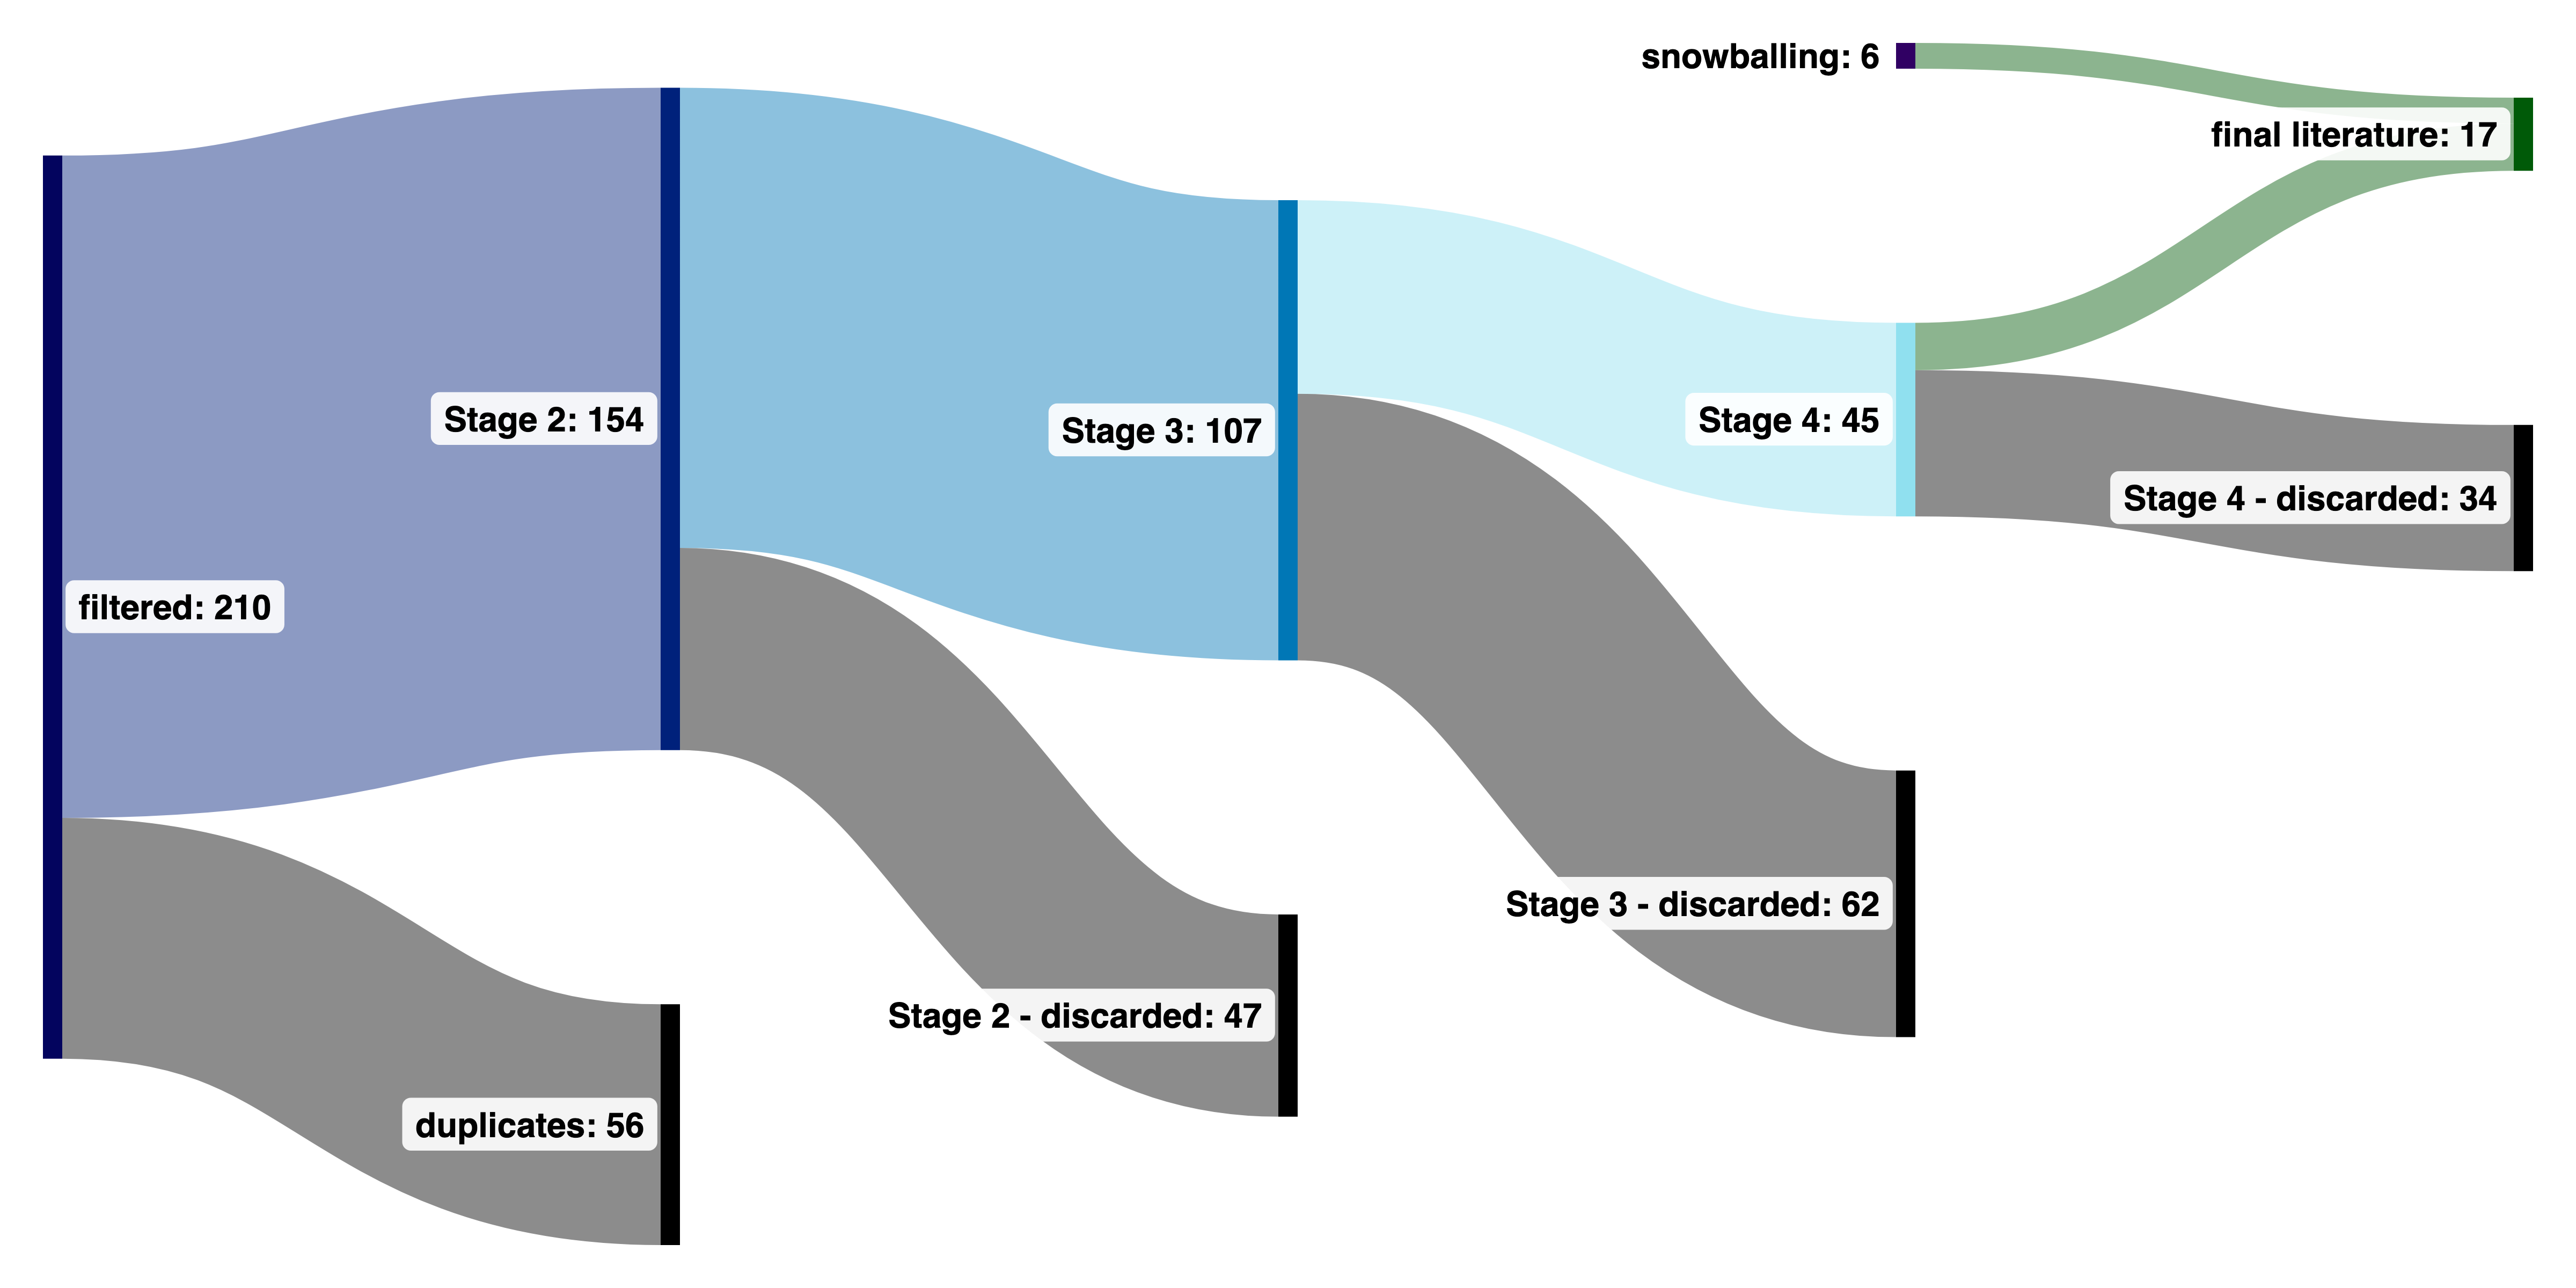
\includegraphics[width=\textwidth]{./2-literature-review/conducting-the-search}
    \caption{Visualization of the subsequent steps of inclusion screening.}
    \label{fig:conducting-the-search-vis}
\end{figure}

In the end, 17 articles were identified during the search.
Figure~\ref{fig:conducting-the-search-vis} summarizes the process.



\section{Discussion of results}\label{sec:evaluation-discussion-of-results}

This section puts the results of the evaluation in a broader context.

\subsection{Conclusions}\label{subsec:conclusions}

Based on data presented in section~\ref{sec:results-of-evaluation} and interpreted in section~\ref{sec:analysis-of-results}, it is possible to answer the RQ2: \enquote{to what extent existing abstract representations of user interfaces can be considered expressive?}
In general, the evaluated UI representations are not particularly expressive \textendash\ certainly not to the point where they could be used to create full-fledged, production-quality applications.
While many representations achieved satisfying results in some areas of UI development outlined earlier, none of them performed well in all areas which limits their potential for use in development.

OpenUIDL was the only representation that achieved substantial scores in two areas (architecture and appearance) and moderate scores in two other areas (behavior and component support).
The language does not yet look like a viable alternative for conventional development, though the technical gap that would need to be closed in order to make it possible is quite narrow \textendash\ the only thing necessary would be a robust mechanism for defining, accessing and mutating state in components and views.
In its current form, it looks more suited for creating high-fidelity prototypes, especially thanks to its extensive styling capabilities.
Even with very simple capabilities of specifying behavior, it might be a replacement for prototyping tools that do not accommodate for interactivity.

In the area of architecture and overall structure, the necessary support was usually present.
Although concepts such as application or modularization are not strictly necessary for creating a functional description, they might be unavoidable for representations that intend to accommodate larger projects.
% todo: \todo{shouldn't this go to future research?}Adding support for dialogs and other non-standard views could also be a relatively low-hanging fruit when it comes to increasing the expressiveness of the notations
Lack of support for logic is probably one of the biggest factors limiting the expressiveness the evaluated representations, not without a reason \textendash\ the solution would need to successfully incorporate concrete code in an otherwise abstract description.
The evaluated notations employed some techniques, such as creating or extending a model of code or integrating with existing code (in fragments or on a larger scale) and, according to the theoretical evaluation, they show substantial results.
% todo: get ready to rewrite this
On the other hand, the limitation to supporting a broad range of components and appearance properties seems to be more conceptual than technical \textendash\ to overcome it, it is simply necessary to formulate a more detailed model.

%\paragraph{Internationalization}
%% \todo{chyba ze to jest w ktoryms z jezykow? idk}
%Many production-grade applications require to be available in more than one language version.
%However, to generate multiple versions of an application`, each using a different language would be impractical;
%instead, any locale-dependent resources (primarily text) are stored outside application code and loaded during runtime, depending on the language set by the user/system.
%Integrating such a mechanism directly into the language would increase the value and flexibility of languages.



%\paragraph{Dependency management}
%As the languages are not mature and widespread, there is little incentive to create, disseminate and manage reusable pieces of UI description.
%Therefore, there are not any mature mechanisms for managing any external dependencies or libraries comparable to what is available for conventional programming languages.
%
%\paragraph{Code integration}
%Currently, the languages presented are limited in their expressiveness by their limited set of actions that can be performed in response to events.
%While it might be a welcome simplification for people unfamiliar with programming, it poses a grave limitation for developers.
%It might be reasonable to accommodate for any gaps in the language by allowing to \enquote{patch} them with code instead.
%
%% \subparagraph{Component lifecycle support}
%% The languages could create a generic lifecycle and support it.
%
%\paragraph{Global application state}
%Most modern GUI programming enhances the event-driven paradigm with the principle of unidirectional data flow: events \enquote{flow} up (events from children components are handled by parent elements) and state \enquote{flows} down (parent components set the state of child components).
%While the principle helps make the components reusable, testable and simpler to a certain extent, it fails in the case where data needs to be available throughout the application.
%The response to this problem are \emph{state containers} that centralize the application state, making state management more predictable and flexible.
%Future iterations of UIDLs could integrate these solutions to increase the flexibility and maintainability of developed applications.


%Conclusions about sections:
%\begin{itemize}
%    \item components \textendash\ the more, the better, and theres no going around that!
%    \item \todo[inline]{include the description of missing components here!}
%    \item appearance \textendash\ similarly!
%\end{itemize}



%components:
%\begin{itemize}
%    \item
%\end{itemize}

%\paragraph{Specialized widgets}
%As mentioned in the previous section, it is desirable for developers/modellers to work with a wide selection of components that neatly fit many possible use cases instead of developing them themselves.
%Unfortunately, they might find the current state of the descriptions lacking, with only the most basic variants of components available in the descriptions.
%For example, in some languages it is possible to use a grid layout;
%however, none of the languages seems to have a masonry layout\footnote{Masonry layout displays content in columns, but unlike a grid, it does not require the conent to be aligned in the row axis, which makes the arrangement more balanced.} defined.
%
%%\subparagraph{(Paged) documents}

% -----

%% \paragraph{Accessibility} \todo{not really sure that's a single feature that can be easily included}
%
%\paragraph{Animations}
%While it is possible to create full-scale applications without any animations, they can still make a big difference and transform a satisfactory user experience to an outstanding one.
%Animations are useful for indicating navigation, interaction progress and state changes in a friendly and visually appealing way.
%Without this feature in UIDLs, generated applications might miss out on this subtle aspect of user experience.
%
%\paragraph{Design systems}
%Design systems have emerged as a solution easing the development of various applications across multiple teams by establishing clear and common rules and style guides, defining reusable patterns and components.
%By using them, organizations and companies can spend less time designing and implementing their applications, while achieving reliability and a unified appearance across all their products.
%So far, there seems to be no explicit support for defining any parts of a style guide in the UIDLs analyzed which make them less suitable for large-scale development.
%
%\paragraph{Dynamic appearance}
%% \todo[inline]{different text directions}
%% todo: 4 sure?
%Additionally, any support for making the appearance of some UI elements dependent on component/application state also seems to be largely absent.
%The most important application for such a feature would be implementation of application themes (especially the famous dark theme).
%This further prevents developers from implementing more engaging interactions and customizable experiences.

% \todo[inline]{maybe write sth nice about the representations? maybe sth surprised you positively? or negatively too!}


\subsection{Limitations of the thesis}\label{subsec:limitations-of-the-study}

% todo: be ready to read this again
The first limitation of the thesis lies in the process of literature review.
Although the process was designed to include as much literature as possible, there might still be relevant UI representations that were not included in the research.
Another limiting factor might be the omission of works published before 2010.

The concepts defined based on the selected literature might not be a sufficiently thorough description of the domain of UIs.
Therefore, the criteria and evaluation method might not produce representative results.
Because the criteria might not have been well-defined, the results might not be objective.
There might be objection to the scoring method \textendash\ maybe not all areas or criteria are equally important and a weighted average would have been more important.

The case study was a minimal example that did not cover all aspects of UI development.
The criteria were simplified to reduce redundancy \textendash\ if we allowed for some redundant requirements, the scores would have been different.
The criteria were also less specific, which could lead to subjectivity.

The evaluation was all the more difficult, as the representations were, for the most part, unavailable beyond their original paper.
There were hardly any specifications, examples or documentation; no way to work with them hands-on.
This made it much more difficult to analyze the notations and draw conclusions.
%\todo[inline]{the representations need to be available, bc otherwise they're useless}

\subsection{Areas for future research}\label{subsec:areas-for-future-research}

Based on the presented conclusions and limitations of the research, multiple directions for future studies can be outlined.

First of all, the criteria and the scoring method proposed in this thesis could be revised and expanded to produce a broader and more accurate judgement of representations.
This development could be based on other existing UIDLs and final UI technologies, possibly including modalities outside the graphical one.
Similarly, the proposed case study and its requirements could be defined in a different way.

Based on the proposed or revised criteria, the evaluation could be repeated with representations chosen in this thesis, with those not included, or even with the ones that do not exist at the time of writing.
This would allow for comparing the established notations with new ones or for comparing the evolution of a given representation across versions.

A more comprehensive and rigorous set of criteria could serve as a reference for researchers and developers of existing or future UIDLs, who could use them to identify gaps in their work.

Finally, the representations could be studied more closely from other angles, such as usability, quality of generated code, etc.

